% !TEX root = ../main.tex
% --+ 11.31 SAMPLING FRACTION ESTIMATION +--------------------------------------
\begin{frame}{Sampling Fraction Estimation}
    \label{11.31::sampling_fraction_estimation}

    To estimate the \ef{sampling fraction} (\% of energy deposited by $e^-$ on calorimeters), we fit \efe{$E_{dep}/p$} distributions in \efe{0.4 GeV $p$} \ef{bins} to
    \begin{empheq}[box={\eqbox[5pt][5pt]}]{equation*}
        f(x) = p_0 \cdot g(x, \mu, \sigma) + p_1 x^2 + p_2 x + p_3,
    \end{empheq}
    where \efe{$g(x, \mu, \sigma)$} is a Gaussian distribution with mean \efe{$\mu$} and standard deviation \efe{$\sigma$}.

    \vspace{-12pt}

    \begin{columns}[onlytextwidth,T]

    \begin{column}{.49\linewidth}
        \begin{center}
            \begin{figure}[t]
                \centering{
                    \fbox{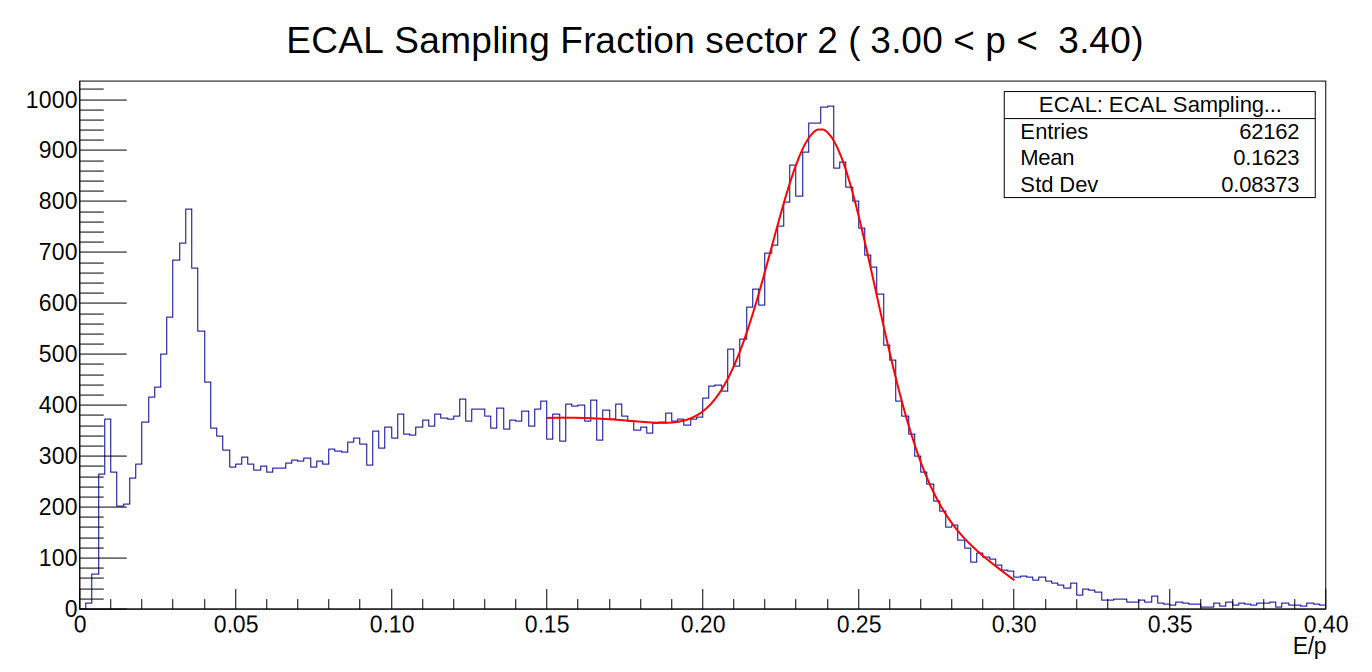
\includegraphics[width=\textwidth]{31sf_1d_plot1.pdf}}
                }
            \end{figure}
        \end{center}
    \end{column}

    \begin{column}{.49\linewidth}
        \begin{center}
            \begin{figure}[t]
                \centering{
                    \fbox{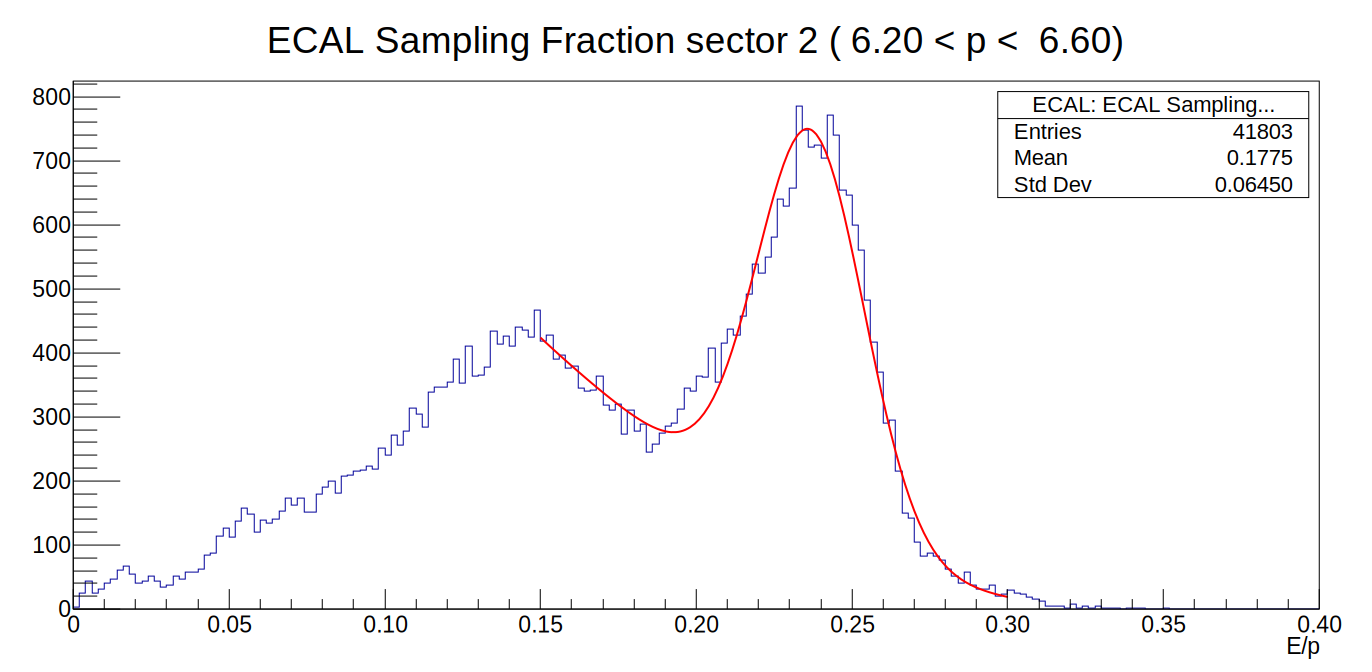
\includegraphics[width=\textwidth]{31sf_1d_plot2.pdf}}
                }
            \end{figure}
        \end{center}
    \end{column}

    \end{columns}

    \vspace{-9pt}

    \scriptsize{\textit{
        \efe{$E_{dep}/p$} distribution for two \efe{$0.4$ GeV $p$} \ef{bins} for $e^-$ in the CLAS12 ECAL.
        The fit only covers from $0.15$ to $0.30$ based on what we expect for $e^-$ from theory.
    }}
\end{frame}

% --+ 11.32 SAMPLING FRACTION ESTIMATION +--------------------------------------
\begin{frame}{Sampling Fraction Estimation}
    \label{11.32::sampling_fraction_estimation}

    The \ef{$\mu$} of each Gaussian fit is then used as data points for a \ef{polynomial fit}, given by
    \begin{empheq}[box={\eqbox[5pt][5pt]}]{equation*}
        f(x) = p_0 \cdot \left(p_1 + \frac{p_2}{x} + \frac{p_3}{x^2}\right),
    \end{empheq}
    which is then used to \ef{correct the energy of $e^-$}.

    \begin{center}
        \begin{figure}[t]
            \centering{
                \fbox{\includegraphics[width=0.8\textwidth]{32sf_2d_plot.pdf}}
            }
        \end{figure}
        \scriptsize{\textit{\ef{$p$} vs. \ef{$E/p$} for $e^-$ in ECAL.}}
    \end{center}
\end{frame}
